\chapter{Podwarstwa Packet Data Convergence Protocol}
\label{cha:pdcp}

\begin{figure}[ht]
	\centerline{\frame{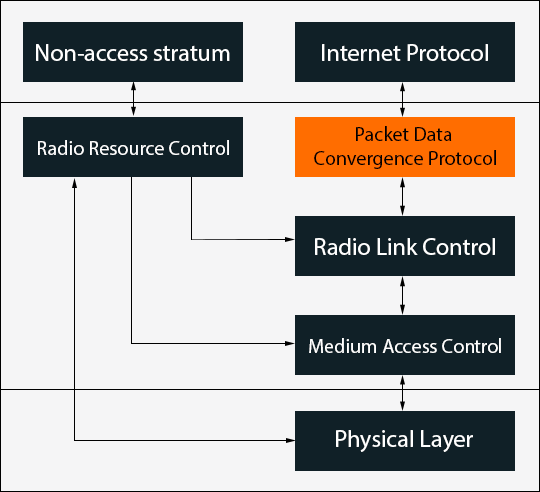
\includegraphics[width=0.5\textwidth]{images/pdcp_overview.png}}}
	\caption{Umiejscowienie podwarstwy PDCP w stosie protokołów LTE}
	\label{fig:pdcpseq}
\end{figure}

Podwarstwa PDCP (Packet Data Convergence Protocol) jest pierwszą z podwarstw z których składa się warstwa 2. stosu protokołów LTE. Dla każdego nośnika radiowego konfigurowana jest jej osobna instancja. Może ona odpowiadać za dane na płaszczyźnie użytkownika (wówczas świadczy usługi dla warstwy IP) lub za dane na płaszczyźnie kontroli i wówczas korzysta z niej warstwa RRC. Warstwa PDCP przesyła pakiety dalej do podwarstwy RLC.

W zależności od płaszczyzny danych, warstwa PDCP jest odpowiedzialna za:

Dla płaszczyzny kontroli:
\begin{enumerate}
	\item Dostarczenie danych w odpowiedniej kolejności i bez duplikatów
	\item Zapewnienie integralności danych
	\item Szyfrowanie danych
\end{enumerate}

Dla płaszczyzny danych użytkownika:
\begin{enumerate}
	\item Dostarczenie danych w odpowiedniej kolejności i bez duplikatów
	\item Kompresję nagłówków
	\item Szyfrowanie danych
\end{enumerate}

W projekcie skupiono się na symulacji przesyłu danych na płaszczyźnie danych użytkownika. Poniżej opisano proces przesyłu pakietu IP od urządzenia użytkownika (UE) do stacji bazowej (eNB) z perspektywy podwarstwy PDCP. Pomocniczo posłużono się zrzutami ekranu z wykonanej symulacji.

\section{Przetwarzanie pakietów IP na podwarstwie PDCP}

\subsection{Nadawanie numeru sekwencyjnego}

Pierwszym krokiem po otrzymaniu pakietu IP z warstwy sieciowej przez podwarstwę PDCP jest nadanie numeru sekwencyjnego. Pozwala on podwarstwie PDCP po stronie odbiornika odrzucić zduplikowane jednostki danych oraz dostarczyć je do wyższych warstw w odpowiedniej kolejności (Rys. \ref{fig:pdcpseq}). 
W tym celu po stronie nadajnika utrzymywany jest liczniki, którego aktualna wartość jest przypisywana jako numer sekwencyjny nowo otrzymanemu pakietowi a następnie inkrementowana. Z kolei po stronie odbiornika odebrane pakiety są umieszczane w buforze gdzie następnie są sortowane na podstawie numeru sekwencyjnego i przekazywane w odpowiedniej kolejności do wyższych warstw.

\begin{figure}[ht]
	\centerline{\frame{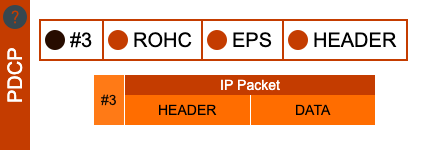
\includegraphics[width=0.5\textwidth]{images/pdcp_1.png}}}
	\caption{Nadanie numeru sekwencyjnego pakietowi IP}
	\label{fig:pdcpseq}
\end{figure}

\subsection{Kompresja metodą ROHC (Robust Header Compression)}

Drugim krokiem jest kompresja nagłówka pakietu IP przy użyciu metody ROHC (Robust Header Compression). Ogólna zasada działania opiera się na założeniu, że jeżeli pakiety IP wysyłane są pomiędzy dwoma urządzeniami wówczas większość pól w ich nagłówkach jest taka sama. W przypadku pakietu IPv4 rozmiar nagłówka wynosi 20 bajtów. Jeżeli jest on użyty w połączeniu z protokołami UDP i RTP wówczas rozmiar nagłówka w sumie wynosi 40 bajtów. ROHC pozwala zmniejszyć rozmiar takiego nagłówka do 2 - 4 bajtów. Warto również zauważyć, że protokół RTP używany zazwyczaj w kodowaniu głosu w czasie rzeczywistym transportuje niewielkie ilości danych w pojedynczym pakiecie - zazwyczaj 20 - 40 bajtów. Porównując to z nieskompresowanym nagłówkiem o ilości 40 bajtów widać, że narzut nagłówka jest znaczny. Dzięki temu zastosowanie kompresji ROHC pozwala zaoszczędzić znaczną część pasma.

\subsection{Szyfrowanie}

Po kompresji następuje szyfrowanie danych zawartych w pakiecie. Zarówno algorytm jak i klucz użyty do szyfrowania jest konfigurowany przez wyższe warstwy. Podczas konstruowania klucza szyfrującego używane są parametry takie jak COUNT (kombinacja numeru sekwencyjnego i numeru ), DIRECTION (kierunek transmisji) oraz parametry dostarczane przez wyższe warstwy, takie jak BEARER (5-bitowy identyfikator nośnika radiowego) oraz KEY (128-bitowy klucz szyfrujący).

\begin{figure}[ht]
	\centerline{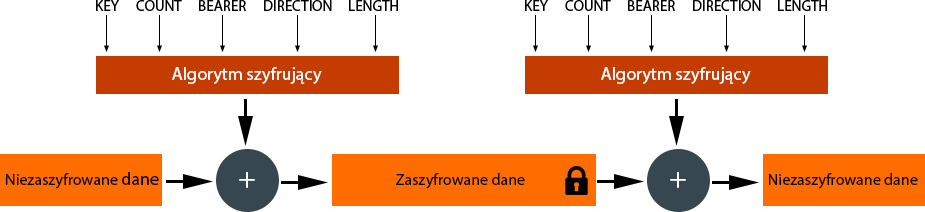
\includegraphics[width=0.9\textwidth]{images/pdcp-eps.png}}
	\caption{Wizualizacja metody szyfrowania danych}
\end{figure}

\subsection{Format wyjściowej jednostki danych (PDU) dla podwarstwy PDCP}

Ostatnim krokiem jest dodanie nagłówków warstwy PDCP i zbudowanie pakietu PDU dla warstwy PDCP. Nagłówek składa się z:
\begin{itemize}
	\item 1-bitowej informacji o tym czy pakiet zawiera dane płaszczyzny użytkownika czy dane płaszczyzny kontroli wygenerowane przez podwarstwę PDCP (pole D/C na rysunkach \ref{fig:pdcp7bit} i \ref{fig:pdcp12bit})
	\item numeru sekwencyjnego zapisanego przy użyciu 7 lub 12 bitów
	\item w przypadku 12-bitowego numeru sekwencyjnego, jest on poprzedzony trzema nieużywanymi bitami zarezerwowanymi do ewentualnego użycia w przyszłości (pola R na rysunku \ref{fig:pdcp12bit})
\end{itemize}

\begin{figure}[ht]
	\centerline{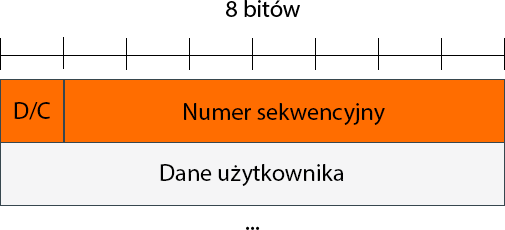
\includegraphics[width=0.4\textwidth]{images/pdcp-pdu-7bit.png}}
	\caption{Pakiet PDU dla warstwy PDCP z 7-bitowym numerem sekwencyjnym}
	\label{fig:pdcp7bit}
\end{figure}

\begin{figure}[ht]
	\centerline{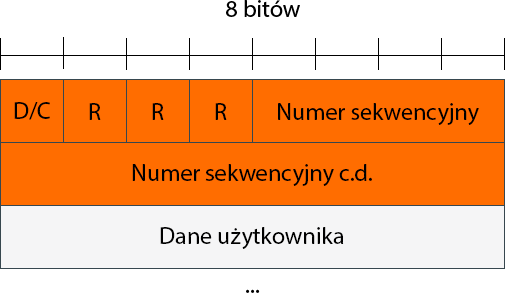
\includegraphics[width=0.4\textwidth]{images/pdcp-pdu-12bit.png}}
	\caption{Pakiet PDU dla warstwy PDCP z 12-bitowym numerem sekwencyjnym}
	\label{fig:pdcp12bit}
\end{figure}